\documentclass{article}


\usepackage{arxiv}

\usepackage[utf8]{inputenc} % allow utf-8 input
\usepackage[T1]{fontenc}    % use 8-bit T1 fonts
\usepackage{hyperref}       % hyperlinks
\usepackage{url}            % simple URL typesetting
\usepackage{booktabs}       % professional-quality tables
\usepackage{amsfonts}       % blackboard math symbols
\usepackage{nicefrac}       % compact symbols for 1/2, etc.
\usepackage{microtype}      % microtypography
\usepackage{lipsum}
\usepackage{graphicx}
\usepackage{amsmath}
\usepackage{amsfonts}
\usepackage{algorithm,algorithmic,bm,color}


\newcommand{\argmin}{\arg\!\min}
%\newcommand{\st}{\mathrm{s.\,t.}}
\newcommand{\Amat}{{\boldsymbol A}}
\newcommand{\Bmat}{{\boldsymbol B}}
\newcommand{\Cmat}{{\boldsymbol C}}
\newcommand{\Dmat}{{\boldsymbol D}}
\newcommand{\Emat}[0]{{{\boldsymbol E}}}
\newcommand{\Fmat}[0]{{{\boldsymbol F}}}
\newcommand{\Gmat}[0]{{{\boldsymbol G}}}
\newcommand{\Hmat}[0]{{{\boldsymbol H}}}
\newcommand{\Imat}{{\boldsymbol I}}
\newcommand{\Jmat}[0]{{{\boldsymbol J}}}
\newcommand{\Kmat}[0]{{{\boldsymbol K}}}
\newcommand{\Lmat}[0]{{{\boldsymbol L}}}
\newcommand{\Mmat}[0]{{{\boldsymbol M}}}
\newcommand{\Nmat}[0]{{{\boldsymbol N}}}
\newcommand{\Omat}[0]{{{\boldsymbol O}}}
\newcommand{\Pmat}[0]{{{\boldsymbol P}}}
\newcommand{\Qmat}[0]{{{\boldsymbol Q}}}
\newcommand{\Rmat}[0]{{{\boldsymbol R}}}
\newcommand{\Smat}[0]{{{\boldsymbol S}}}
\newcommand{\Tmat}[0]{{{\boldsymbol T}}}
\newcommand{\Umat}{{{\boldsymbol U}}}
\newcommand{\Vmat}[0]{{{\boldsymbol V}}}
\newcommand{\Wmat}[0]{{{\boldsymbol W}}}
\newcommand{\Xmat}{{\boldsymbol X}}
\newcommand{\Ymat}[0]{{{\boldsymbol Y}}}
\newcommand{\Zmat}{{\boldsymbol Z}}

\newcommand{\av}{\boldsymbol{a}}
\newcommand{\Av}{\boldsymbol{A}}
\newcommand{\Cv}{\boldsymbol{C}}
\newcommand{\bv}{\boldsymbol{b}}
\newcommand{\cv}{{\boldsymbol{c}}}
\newcommand{\dv}{\boldsymbol{d}}
\newcommand{\ev}[0]{{\boldsymbol{e}}}
\newcommand{\fv}{\boldsymbol{f}}
\newcommand{\Fv}[0]{{\boldsymbol{F}}}
\newcommand{\gv}[0]{{\boldsymbol{g}}}
\newcommand{\hv}[0]{{\boldsymbol{h}}}
\newcommand{\iv}[0]{{\boldsymbol{i}}}
\newcommand{\jv}[0]{{\boldsymbol{j}}}
\newcommand{\kv}[0]{{\boldsymbol{k}}}
\newcommand{\lv}[0]{{\boldsymbol{l}}}
\newcommand{\mv}[0]{{\boldsymbol{m}}}
\newcommand{\nv}{\boldsymbol{n}}
\newcommand{\ov}[0]{{\boldsymbol{o}}}
\newcommand{\pv}[0]{{\boldsymbol{p}}}
\newcommand{\qv}[0]{{\boldsymbol{q}}}
\newcommand{\rv}[0]{{\boldsymbol{r}}}
\newcommand{\sv}[0]{{\boldsymbol{s}}}
\newcommand{\tv}[0]{{\boldsymbol{t}}}
\newcommand{\uv}[0]{{\boldsymbol{u}}}
\newcommand{\vv}{\boldsymbol{v}}
\newcommand{\wv}{\boldsymbol{w}}
\newcommand{\Wv}{\boldsymbol{W}}
\newcommand{\xv}{\boldsymbol{x}}
\newcommand{\yv}{\boldsymbol{y}}
\newcommand{\Xv}{\boldsymbol{X}}
\newcommand{\Yv}{\boldsymbol{Y}}
\newcommand{\zv}{\boldsymbol{z}}

\newcommand{\xvf}{\widetilde{\xv}}
\newcommand{\Fmb}{\boldsymbol{\mathcal{F}}}

\newcommand{\Gammamat}[0]{{\boldsymbol{\Gamma}}}
\newcommand{\Deltamat}[0]{{\boldsymbol{\Delta}}}
\newcommand{\Thetamat}{\boldsymbol{\Theta}}
\newcommand{\Lambdamat}{{\boldsymbol{\Lambda}}}
\newcommand{\Ximat}[0]{{\boldsymbol{\Xi}}}
\newcommand{\Pimat}[0]{{\boldsymbol{\Pi}} }
\newcommand{\Sigmamat}{\boldsymbol{\Sigma}}
\newcommand{\Upsilonmat}[0]{{\boldsymbol{\Upsilon}} }
\newcommand{\Phimat}{\boldsymbol{\Phi}}
\newcommand{\Psimat}{\boldsymbol{\Psi}}
\newcommand{\Omegamat}{{\boldsymbol{\Omega}}}

\newcommand{\Lambdav}{\bm{\Lambda}}
\newcommand{\alphav}{\boldsymbol{\alpha}}
\newcommand{\betav}[0]{{\boldsymbol{\beta}} }
\newcommand{\gammav}{{\boldsymbol{\gamma}}}
\newcommand{\deltav}[0]{{\boldsymbol{\delta}} }
\newcommand{\epsilonv}{\boldsymbol{\epsilon}}
\newcommand{\zetav}[0]{{\boldsymbol{\zeta}} }
\newcommand{\etav}[0]{{\boldsymbol{\eta}} }
\newcommand{\thetav}{\boldsymbol{\theta}}
\newcommand{\iotav}[0]{{\boldsymbol{\iota}} }
\newcommand{\kappav}{{\boldsymbol{\kappa}}}
\newcommand{\lambdav}[0]{{\boldsymbol{\lambda}} }
\newcommand{\muv}{\boldsymbol{\mu}}
\newcommand{\nuv}{{\boldsymbol{\nu}}}
\newcommand{\xiv}{{\boldsymbol{\xi}}}
\newcommand{\omicronv}[0]{{\boldsymbol{\omicron}} }
\newcommand{\piv}{\boldsymbol{\pi}}
\newcommand{\rhov}[0]{{\boldsymbol{\rho}} }
\newcommand{\sigmav}[0]{{\boldsymbol{\sigma}} }
\newcommand{\tauv}[0]{{\boldsymbol{\tau}} }
\newcommand{\upsilonv}[0]{{\boldsymbol{\upsilon}} }
\newcommand{\phiv}{\boldsymbol{\phi}}
\newcommand{\chiv}[0]{{\boldsymbol{\chi}} }
\newcommand{\psiv}{\boldsymbol{\psi}}
\newcommand{\omegav}[0]{{\boldsymbol{\omega}} }

\newcommand{\tsp}{^{\mathsf{T}}}
\newcommand{\inv}{^{-1}}
\newcommand{\ie}{{\em i.e.}}
\newcommand{\st}{{\em s.t.}}
\newcommand{\eg}{{\em e.g.}}
\newcommand{\wrt}{{\em w.r.t.\,}}
\DeclareMathOperator{\mst}{s.t.}


\title{Dimensionality Reduction}


\author{
  Haoqi~Zhang\\
  \And
  Kaiqi~Jin\\
  \And
  Peihao~Yang\\
  \texttt{516021910233} \\
  \And
  Yi~Zhang\\
}
  
\begin{document}
\maketitle

\begin{abstract}
In this report, we first use support vector machine (SVM) to classify 37322 images with 2048 pre-extracted deep learning features for each image. The data is from the Attributes (AwA2) dataset~\cite{AwA2}. We then reduce the dimensionality in different way and make classification with SVM again. The experiments show that some dimensionality reuction methods are efficient and reliable.
\end{abstract}


% keywords can be removed
\keywords{Dimensionality reduction \and Feature selection \and Feature projection \and Feature learning}


\section{Introduction}
Since the information revolution last century, more and more data has been generated. The dimension curse gradually becomes a critical problem in data science. The last decades have seen plenty of methods to reduce the dimensionality of the data. 

In this report, we will divide reduction methods into three classes, and discuss them based on solid experiment results. The first kind of reduction methods is feature selection, which means that we directly select important features from raw data to reduce the dimensionality, such as variance threshold based selection (VT), genetic algorithm(GA), and so on. The second one is feature projection, which means that we can apply reduction by projecting original features to a low dimensionality space without much loss of information, such as principle component analysis (PCA), linear discriminant analysis (LDA). The last but not least, we will introduce some nowadays prevalent methods based on feature learning, such as t-distributed stochastic neighbor embedding (TSNE), random forest (RF), local linear embedding (LLE) and so on.

Support vector machine (SVM) is a classical method often applied in the classification tasks~\cite{SVM}. By introducing the kernel trick, the SVM could overcome the limits of linear model, and be applied to non-linear problems~\cite{}. We will analyse several kinds of kernel SVM and compare their classification ability on AwA2 dataset.

The Section~\ref{sec:baseline} is the leadin. We will introduce the assessment baseline and assessment criterions applied. The dimensionality reduction methods would be covered in the next three section. In Section~\ref{sec:selection}, we introduce the feature selection methods in detail. We analysis the feature projection methods in Section~\ref{sec:projection}. The feature learning methods are discussed in Section~\ref{sec:learning}. The experiment results and comparisons are in the Section~\ref{sec:discussion}.  In the end, a thorough conclusion is made.


\section{Baseline}
\label{sec:baseline}
\subsection{Theory}
To analyse the effect of the dimensionality reduction methods, we have to set a baseline as a comparison. We select recommended linear SVM as our baseline model. Linear SVM solve the following primal problem
\begin{equation}
	\label{eq:lsvm}
	\begin{split}
		\min~&\frac{1}{2} \wv^T\wv + C\sum_{i=1}^{N} \epsilon_i\\
		\mst~&y_i(\wv^T\xv_i+b)\geq 1-\epsilon_i\\
		     &\epsilon_i\geq0, i =1,\ldots,N.
	\end{split}
\end{equation}

And the dual problem is
\begin{equation}
	\label{eq:lsvm_d}
	\begin{split}
		\min~&\frac{1}{2} \alphav^T\Qmat\alphav-\ev^T\alphav\\
		\mst~&\yv^T\alphav=0\\
			 &0\le\alphav_i\ge C, i=1,\ldots,N,
	\end{split}
\end{equation}
where $\Qmat_{ij}$ is $y_iy_jx_i^Tx_j$, and $\ev$ is a unit vector of size $n\times1$. 

However, we also make experiments on other kinds of SVM with different kernel function to compare their classification abilities. And we compare several kernel functions, such as,
\begin{enumerate}
	\item linear kernel function~~$<x,x'>$,
	\item polynomial kernel function~~$(\gamma<x,x'>+r)^d$,
	\item radial basis kernel function~~$\exp(-\gamma\|x-x'\|^2)$,
	\item sigmoid kernel function~~$\tanh(\gamma<x,x'>+r)$.
\end{enumerate}

With kernel function, the primal problem of SVM becomes
\begin{equation}
	\label{eq:svm}
	\begin{split}
	\min~&\frac{1}{2} \wv^T\wv + C\sum_{i=1}^{N} \epsilon_i\\
	\mst~&y_i(\wv^T\phi(\xv_i)+b)\geq 1-\epsilon_i\\
	&\epsilon_i\geq0, i =1,\ldots,N.
	\end{split}
\end{equation}

And the dual problem is
\begin{equation}
	\label{eq:svm_d}
	\begin{split}
	\min~&\frac{1}{2} \alphav^T\Qmat\alphav-\ev^T\alphav\\
	\mst~&\yv^T\alphav=0\\
	     &0\le\alphav_i\ge C, i=1,\ldots,N,
	\end{split}
\end{equation}
where $\Qmat_{ij}$ is $y_iy_jK(x_i,x_j)$, $K(x_i,xj)$ is the kernel function and $\ev$ is a unit vector of size $N\times1$. 

\subsection{SVM parameter setting}
The experiment results will be discussed in the Section~\ref{sec:discussion}. Here, we just describe the experiment process in detail. For baseline implementation, we use the scikit-learn library~\cite{sklearn}. We split the dataset into training set and test set with a proportion of $3:2$, which means that $60\%$ of the AwA2 data is used to train the SVM model. After trying different values as shown in Figure~(\ref{fig:lSVM}), we finally build our linear SVM model with $C=0.01$.

As shown in Figure~(\ref{fig:lSVM}), we select two criterions, accuracy score and f1-score, to compare the accuracy of SVMs. We will continue using these two in the following experiments. The accuracy score $s_1$ is defined by
\begin{equation}
	\label{eq:score}
	s_1 = \frac{\sum_{i=1}^{N}\hat{y_i} == y_i}{N},
\end{equation}
where $\hat{y_i}$ is the predicted label for $i-th$ data.

And the f1-score $s_{2k}$ for class $k$ is defined by
\begin{equation}
	\label{eq:f1-score}
	\begin{split}
	&s_{2k} = \frac{2P_k*R_k}{P_k+R_k},\\
	&P_k = \frac{TP_K}{TP_k+FP_k},\\
	&R_k = \frac{TP_k}{TP_k+FN_K}
	\end{split}
\end{equation},
where $P$ is the precision, $R$ is the recall, $TP$ is true positive amount, $FP$ is false positive amount, $FN$ is the false negative amount.

\begin{figure}
	\label{fig:lSVM}
	\caption{Set different parameter for linear SVM}
	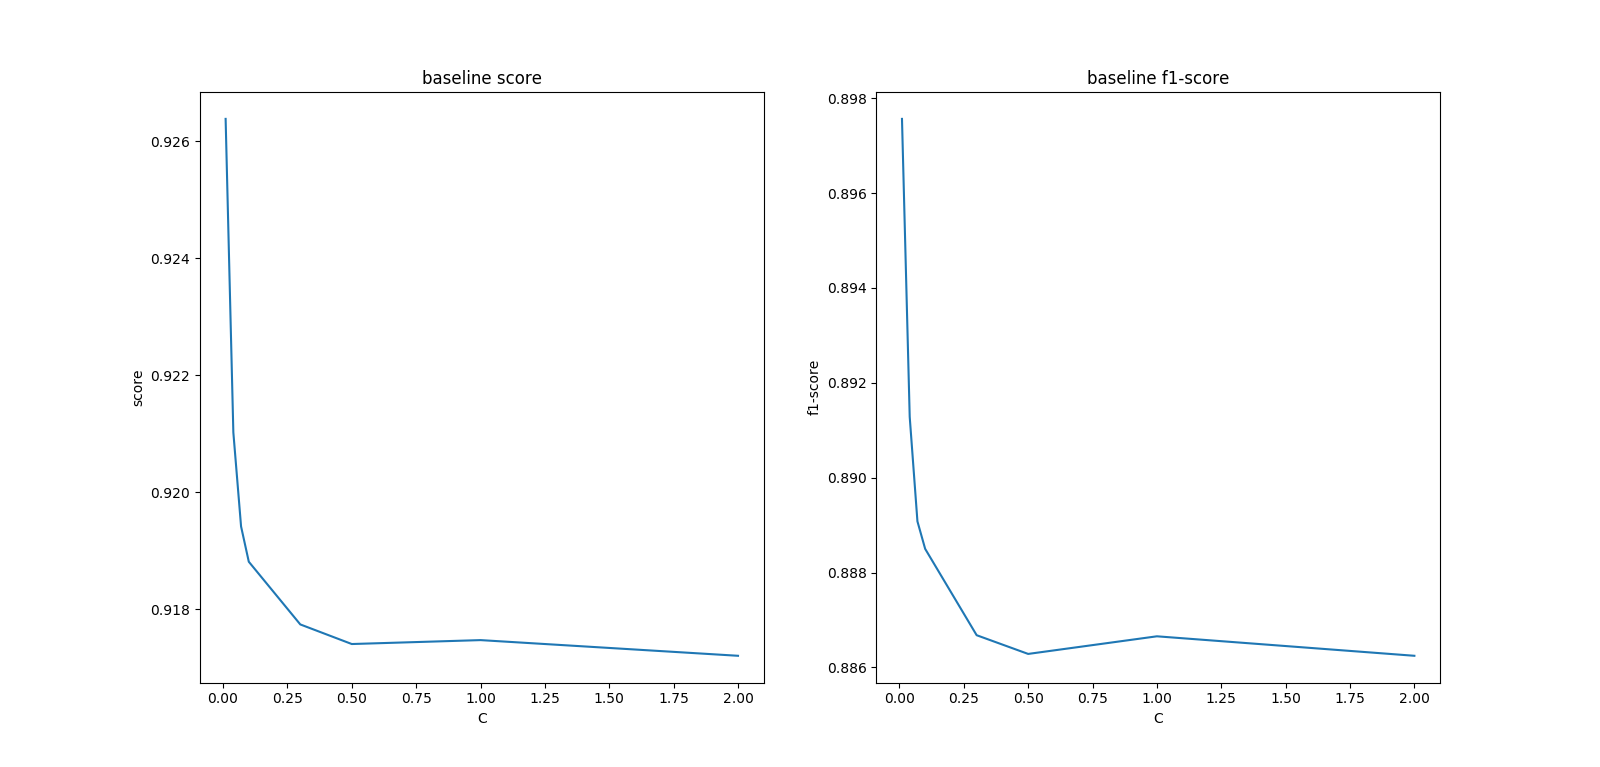
\includegraphics[width=\linewidth]{figs/baseline.png}
\end{figure}

The experiment results with different kernel functions are shown in the Figure~(\ref{fig:SVM}). We can find linear SVM nearly always outperforms others on the AwA2 dataset with arbitary parameter $C$. And linear SVM is much faster and smaller than any other kind of SVM. So it's reasonable that the linear SVM is recommended in the tutorial. It seems that the linear SVM is more robust than SVM with other kernels despite what the parameter $C$ is.

The "ovo" in Figure~\ref{fig:SVM} means "one-vs-one" and "one-vs-rest" for multi- class classification~\cite{}. For "one-vs-one", if $K$ is the number of classes, then $K * (K - 1) / 2$ classifiers are constructed and each one trains data from two classes. As for "one-vs-rest", only $K$ classifiers are constructed. The result is similar for the both kind of classifiers. To reduce the calculation, we use "ovr" in our baseline linear SVM.

\begin{figure}
	\label{fig:SVM}
	\caption{Different SVM kernels.}
	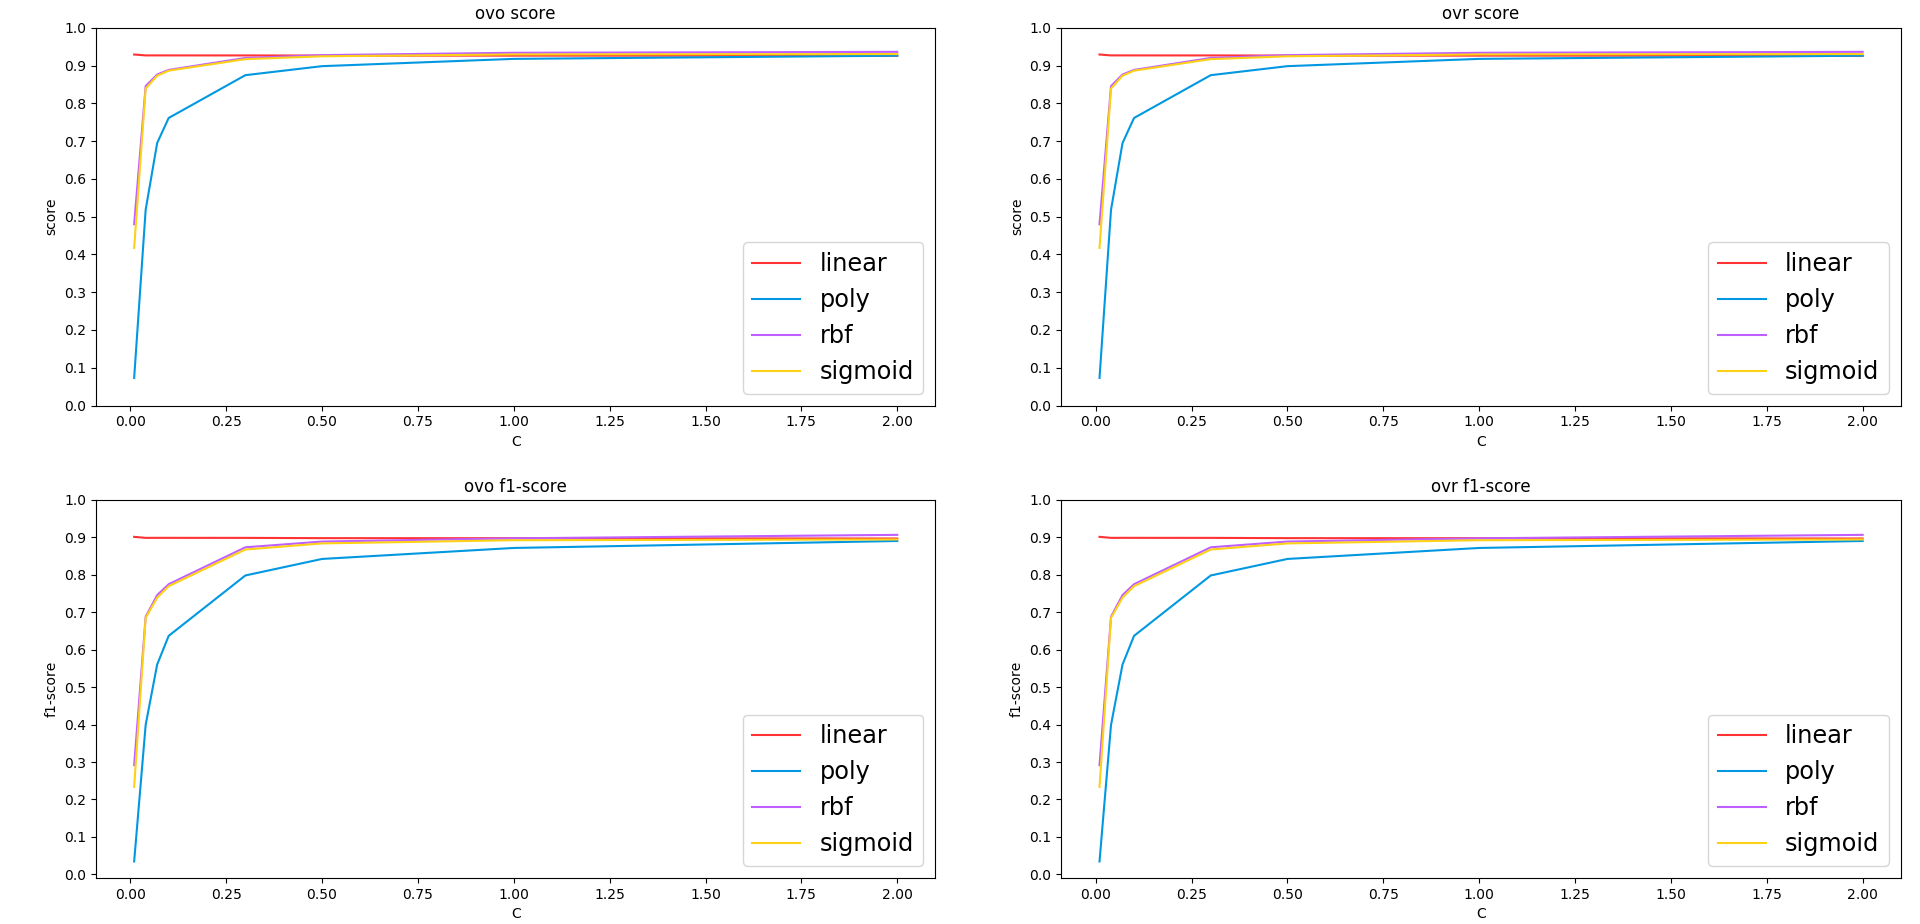
\includegraphics[width=\linewidth]{figs/compare.png}
\end{figure}


\section{Feature selection}
\label{sec:selection}
Feature selection is a kind of methods that directly select some features from the original data. The core of these methods are often the selection criterion. The thought of feature selection is simple but they are efficient and reliable. We tried plenty of algorithms such as variance threshold based selection (VT), univariate feature selection (UF), selecting from model (SFM), calculating the area under the ROC curve (AUC\_ROC) and genetic algorithm (GA).

\subsection{Variance Threshold}
The variance threshold based selection is in fact a kind of backward selection method. It removes all of the features whose variance can't reach a specific threshold. For example, if the feature is the same for every sample, obviously it is useless for classification task and it should be removed. The larger the threshold is, the less features remain. We tried $50$ kinds of threshold to draw a curve to show the relationship between accuracy and variance threshold (feature number) in Figure~\ref{fig:complete}. It could be described as the Algorithm~\ref{alg:vt}.

\begin{algorithm}
	\caption{VT}
	\label{alg:vt}
	\begin{algorithmic}[1]
		\REQUIRE Variance threshold $v$, set of all the features $U$, feature amount $F$, data samples $\Xmat$ of size $N\times F$.
		\ENSURE Selected features $S$.
		\STATE Initialize $S=U$.
		\FOR{$f=1,...,F$}
			\IF{$Variance(\Xmat[:,f])<v$}
				\STATE $S = S-{f}$.
			\ENDIF
		\ENDFOR\\
		\RETURN $S$
	\end{algorithmic}
\end{algorithm}

\subsection{Univariate Feature}
This is a forward selection method. We test $12$ different feature amounts to draw the Figure~\ref{fig:complete}. The univariate feature selection is based on univariate statistic tests. It always select the features dependent on the label statistic. Here we use chi-square tests to describe the dependence between feature and label. If a statistic is dependent upon another one, the chi-square value $\chi^2$ between them will be very large. So we simply select the features with larger chi-square value denoted $\chi^2(\xv,\yv)$. This can be described in Algorithm~\ref{alg:uf} detailedly.

\begin{algorithm}
	\caption{UF}
	\label{alg:uf}
	\begin{algorithmic}[1]
		\REQUIRE Desired feature amount $V$, set of all the features $U$, feature amount $F$, data samples $\Xmat$ of size $N\times F$.
		\ENSURE Selected features $S$.
		\STATE Initialize $S=U$.
		\FOR{$f=1,...,F$}
			\STATE $\chiv[f] = \chi^2(\Xmat[:,f],\yv)$.
		\ENDFOR\\
		\STATE Sort the $\chiv$ array in descending order.
		\STATE Select the top $V$ features.
		\RETURN $S$
	\end{algorithmic}
\end{algorithm}

\subsection{Select From Model}
This is a backward selection method. Since we already build a SVM in the experiment above, here is another method directly use the information of SVM to reduce the dimensionality. The scikit-learn library uses logistic function to map an output to the interval $(0,1)$ as Equation
\begin{equation}
	\label{eq:coef}
	h(x) = \frac{1}{1+\exp^{-\thetav^Tx}}
\end{equation}
shows. And it uses a parameter called $SVM.\_coef$ to record the $\thetav$ in the logistic function for classification. We can treat this $\thetav$ as a vector of weighting coefficients. Little weighting coefficient indicates little influence to the classification. So we could select features according to the coefficients. We have to assign a threshold or the desired feature number for the importance. The algorithm is similar to VT or UF, and we also set $12$ different value to get the curve in the Figure~\ref{fig:complete}.


\subsection{Area Under Curve ROC}
This is a forward selection method. This method is similar the univariate feature selection, the difference is the selection criterion is not the dependent degree, but the area under the curve of receiver operating characteristic (AUC\_ROC). 

The ROC is kind a curve that measure the ability of classifier. Recall the true positive (TP), false positive, true negative (TN) and false negative (FN) mentioned above. We further define the false positive rate (FPR) and the true positive rate (TPR), where
\begin{equation}
	\label{eq:roc}
	\begin{split}
		&FPR = \frac{FP}{TN+FP},\\
		&TPR = \frac{TP}{TP+FN}.
	\end{split}
\end{equation} 
The axis of ROC is labelled by FPR and TPR. The AUC won't larger than $1$, since the FPR and TPR are both smaller than $1$. A good classifier is with lower FPR and higher TPR. That is, the AUC of the ROC should be as large as possible. So we first calculate the AUC\_ROC of every feature independently, then select features with higher AUC\_ROC values. 

\subsection{Genetic Algorithm}
The AwA2 dataset is so large that we can't run genetic algorithm (GA) directly on it. But we still analysis it and test it on a part of the AwA2 dataset. We think GA is not a good idea under this circumstance, because of the fact that it need to utilize too much calculation resource considering the frequent assessment of gene fitness and crossing over. What's more, an encoded gene (here we encode a gene with one-hot code of features) is too long, it doesn't solve the combination explosion problem even we can reduce the searching space slightly with fitness function in GA. Moreover, how to define a good fitness function is another knotty problem.


\section{Feature projection}
\label{sec:projection}
\subsection{Principal Component Analysis}
\subsubsection{Theory of PCA}
    The process of PCA can be summarized as a linear mapping of feature vectors to a lower-dimensional space, where the linear correlation among variables are minimized, in the lower-dimensional space the features are almost independent with others and thus could make the classification easier and avoid the overfitting problem. To achieve such low-dimensional independent features, there are two ways, the first way is to find the maximum variance direction as our new main dimension since different features are very different in this direction. The other way is try to minimize the reconstruction error since after pca we will lose some data and we wan't to preserve as many data as possible. However these two methods are equivalent iin mathematics.
    
    Consider $n$ feature vectors (which is37322) each of dimension $p$ (which is 2048 in our project), whole PCA process is as follows:
\begin{enumerate}
\item Centralize our data to make the average value of each feature become 0
\begin{equation}
	x_i =x_i- \frac{1}{n} \sum_{i=1}^n x_i\label{eq:mean}
\end{equation}

\item Calculate the covariance matrix $C$ from the samples with
\begin{equation}
	C = \frac{1}{n-1} \sum_{i=1}^n x_i x_i^T - u u^T \label{eq:cx}
\end{equation}

\item Compute the eigenvectors and eigenvalues of the covariance matrix $C$.
\begin{equation}
	V^T CV = D \label{eq:eig}
\end{equation}
	where the matrix $V$ consists of eigenvectors which diagonalizes the covariance matrix $C$, and $D$ is the diagonal matrix of eigenvalues of $C$.

\item Rearrange the eigenvectors and eigenvalues in a way that the columns of the eigenvector matrix $V$ and eigenvalue matrix $D$ are sorted in order of decreasing eigenvalue. The eigenvalues represent the distribution of the source data's energy among each of the eigenvectors, where the eigenvectors form a basis for the data.

\item Select the first $k$ columns of $V$ as the $p \times k$ matrix $W$, 

\item Project the original data onto the new basis. After reduced the dimension of our data, we can move to the classification part.
\begin{equation}
	t_i = W^T (x_i - u)\label{eq:proj}
\end{equation}

\end{enumerate}
\subsubsection{Experiment result and analysis}
We have used sk-learn library of python when doing our PCA. We have tried many components in this experiment and finally we get the final result which is shown in the table \ref{tab:pca}. One main problem is that no matter how we adjust our $k$, our result is always not as good as the baseline. After analysis, we found that this is because the features we use are not raw features, and they come from the ResNet101, which means they have already been processed by the network. So, we think all of these features contains some kind of information which is essential for the classification, and there is little redundant feature. Our PCA process will discard some of them to achieve a lower-dimensional feature, so the result will be slightly worse than the baseline. This explains why that when the number of $k$ (the dimension of our new feature vector) is very high, the performance is almost as good as the baseline, and when $k$ is relatively small, the performance of the pca will become quite bad. So, after trying we found when $k$ is about 500, the PCA can get the best performance which means it can use less features to achieve the best SVM classification accuracy . More details are shown in \ref{fig:pca_score} .
\begin{table}
	\centering
	\caption{Performance with different k in PCA}
	\label{tab:pca}
	\begin{tabular}{lccccccccccc}
		
		\specialrule{0em}{1pt}{1pt}
		k-num&1024 &640&576&434&256&128&64&32&16&8&2\\
		\hline
		\hline
		\specialrule{0em}{1pt}{1pt}
		score &0.922&0.925&0.924&0.922 &0.923&0.914&0.897&0.861&0.776&0.614&0.190\\
		\hline
		\specialrule{0em}{1pt}{1pt}
		F1-score &0.892&0.894&0.893&0.890 &0.889&0.869&0.840&0.764&0.652&0.460&0.074\\
		
		\hline
	\end{tabular}
\end{table}

\begin{figure}[htbp]
	\centering
	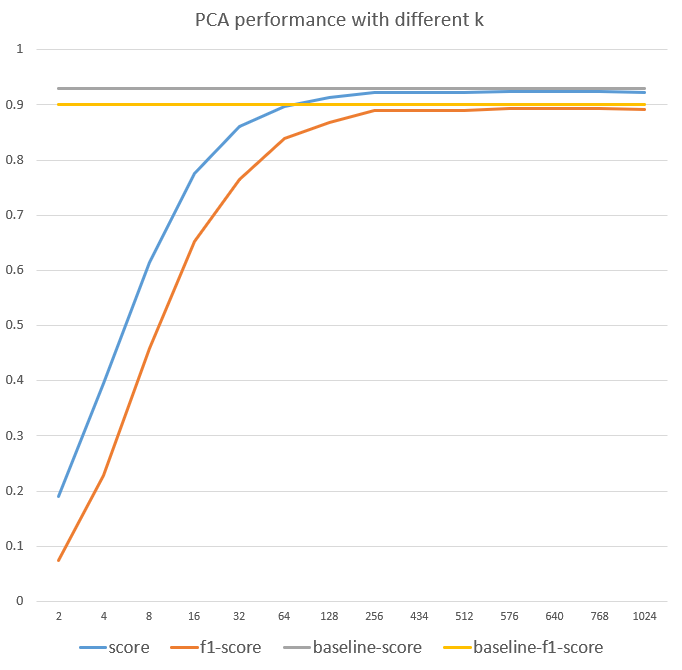
\includegraphics[width=0.45\linewidth]{figs/pca2.png}
	\caption{PCA performance with different k }
	\label{fig:pca_score}
\end{figure}



\subsection{Linear Discriminant Analysis}
\subsubsection{Theory of LDA}
	LDA is the Linear Discriminant Analysis, which is similar to PCA since both of them are feature projection methods and both of them try to convert the original high-dimensional feature into a new low-dimensional space. But there are some differences between them. LDA want to find a low-dimensional space which can maximize the class separation of the samples, thus it needs the label of each sample to reduce the dimensionality. And the number of labels will have great effect on the final result of LDA. The computational procedurel of LDA is as follows.
	
	Consider $n$ feature vectors (which is37322) each of dimension $p$ (which is 2048 in our project) and there are 50 labels in total, 
\begin{enumerate}
\item Calculate the scatter matrix $S_w$ of each class.

\item Calculate the scatter matrix $S_w$  between different class.

\item Calculate $S^{-1}_wS_b$ and compute the eigenvectors and eigenvalues of it just like PCA

\item Rearrange the eigenvectors and eigenvalues in a way that the columns of the eigenvector matrix $V$ and eigenvalue matrix $D$ are sorted in order of decreasing eigenvalue. The eigenvalues represent the distribution of the source data's energy among each of the eigenvectors, where the eigenvectors form a basis for the data.

\item Select the first $k$ columns of $V$ as the $p \times k$ matrix $W$, 

\item Project the original data onto the new basis. 
\begin{equation}
	t_i = W^T x_i \label{eq:proj}
\end{equation}

\end{enumerate}

\subsubsection{Experiment result and analysis}
We have used sk-learn library of python to do LDA. We tried a lot of components of $k$ when finding the best setting of LDA. We found that when $k$ is close to the number of label classes (which is 50 in this dataset), the result will be good. However, when $k$ becomes bigger than 50., the result will have no improvement. We thought it's just because we are creating our new space based on our feature classes and when $k$ is bigger than 50, there is no space for us to further improve the class separation. When $k$ is small, similar to PCA, the performance of our SVM will become quite bad, it is also obvious since it have lost a lot of information. Similar to PCA, since LDA discarded some information compared with the original feature, our final result is slightly worse than the baseline. More details are shown in \ref{fig:lda_score}.
\begin{table}
	\centering
	\caption{Performance with different k in LDA}
	\label{tab:pca}
	\begin{tabular}{lccccccccccc}
		
		\specialrule{0em}{1pt}{1pt}
		k-num&2&4&8&12&16&24&32&40&48&50&58\\
		\hline
		\hline
		\specialrule{0em}{1pt}{1pt}
		score &0.197&0.327&0.497&0.630 &0.698&0.814&0.861&0.900&0.923&0.923&0.923\\
		\hline
		\specialrule{0em}{1pt}{1pt}
		F1-score &0.085&0.185&0.328&0.453 &0.531&0.667&0.745&0.818&0.884&0.893&0.893\\
		
		\hline
	\end{tabular}
\end{table}
	
\begin{figure}[htbp]
	\centering
	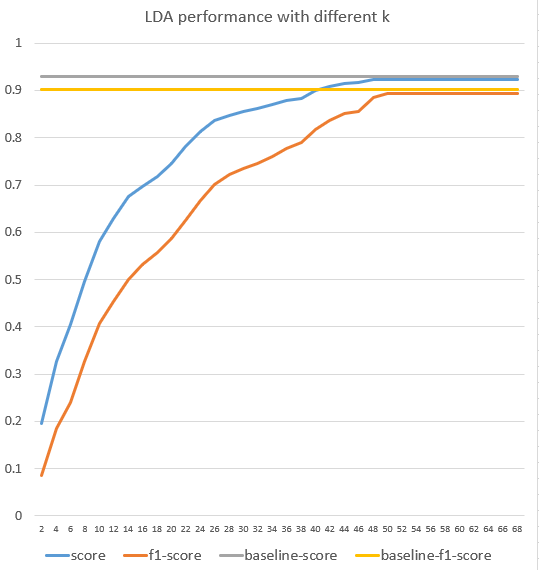
\includegraphics[width=0.45\linewidth]{figs/lda.png}
	\caption{LDA performance with different k }
	\label{fig:lda_score}
\end{figure}






\section{Feature learning}
\label{sec:learning}

\section{Discussion}
\label{sec:discussion}
\subsection{Reduction on the complete dataset}
Most dimensionality reduction experiments were carried on the complete AwA2 dataset. We changed the number of selected features or other parameters to control the degree of the reduction, and then train linear SVMs on these reduction results. The criterions for the SVM predictions, as mentioned before, are the f1-score and mean accuracy. The comparison is shown in Figure~(\ref{fig:complete}). The red line is the linear SVM baseline.
  \begin{figure}
  	\label{fig:complete}
  	\caption{Comparison on the AwA2 dataset.}
  	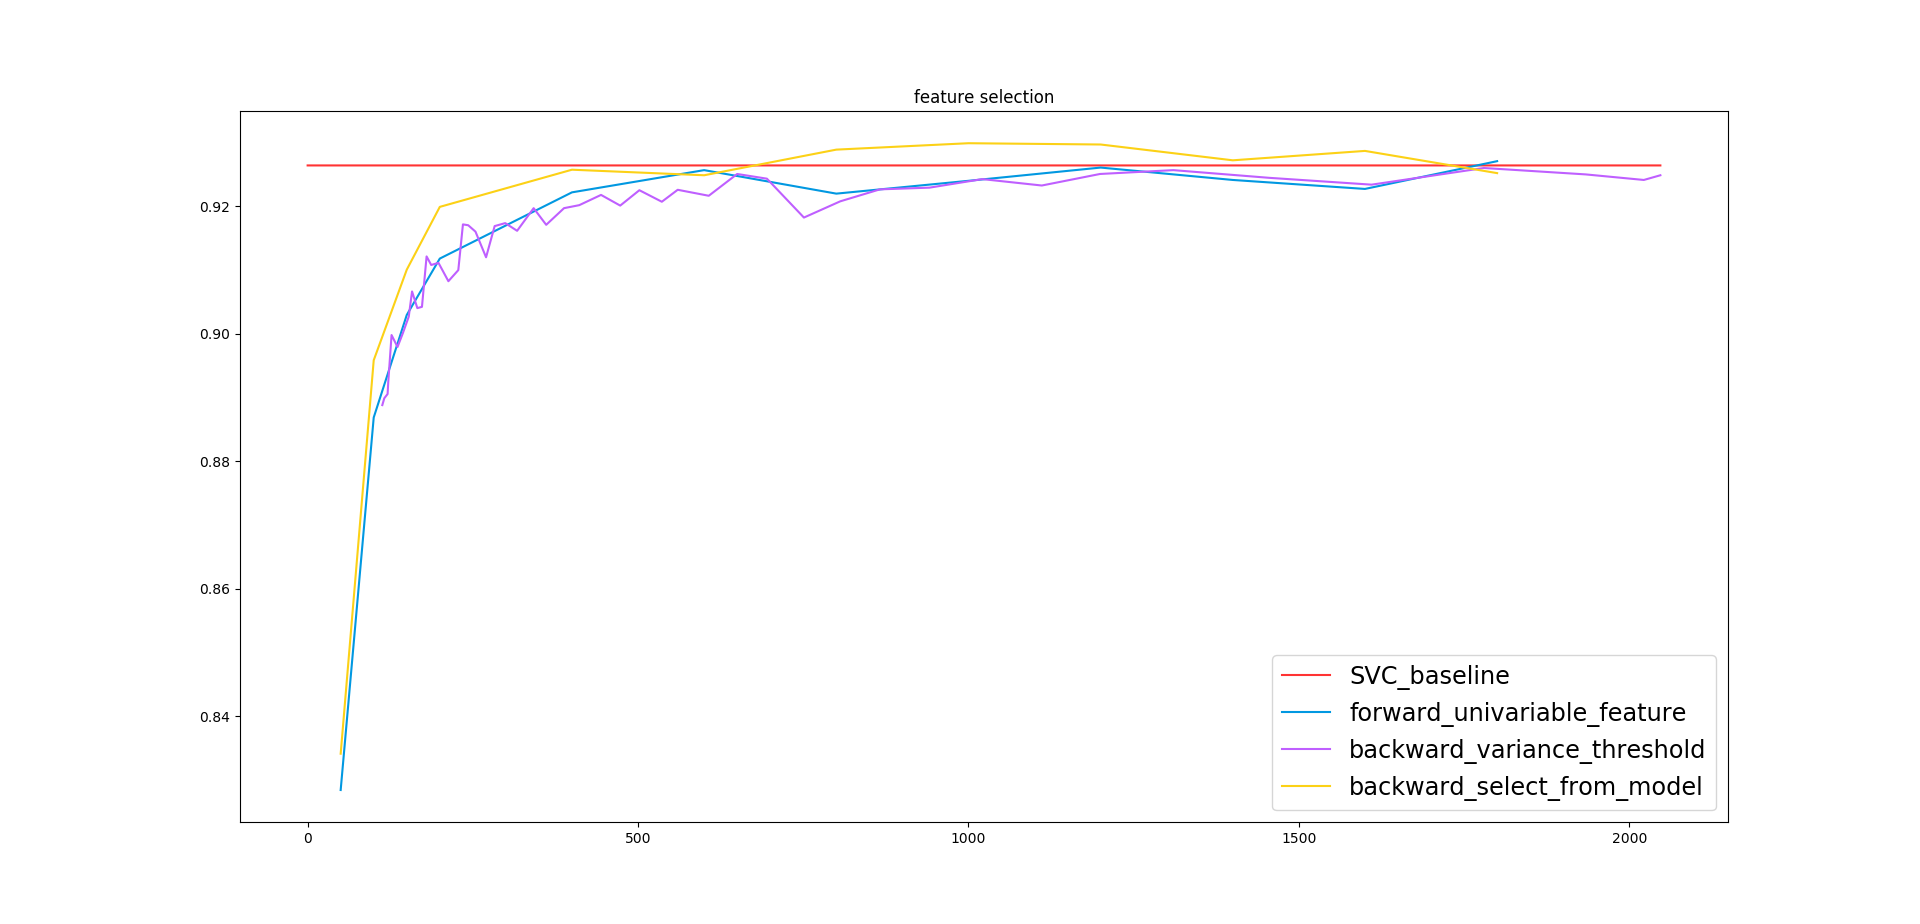
\includegraphics[width=\linewidth]{figs/feature_selection.png}
  \end{figure}

\subsection{Reduction on the smaller dataset}
As mentioned before, the AwA2 dataset is too large for some reduction methods, so we made experiments on a smaller dataset to verify the effectiveness of these methods. This smaller dataset was selected from the AwA2 dataset.

\section{Conclusion}

\bibliographystyle{unsrt}  
\bibliography{references}


\end{document}